\chapter{Properties of schedule DAGs and optimal schedules}
\label{chap:p3}

We now researching some properties of snapshot DAGs and optimal schedules. In particular, we will look at a particular non-trivial class of intrees, for which HLF is optimal.

\section{Properties of optimal schedules}
\label{sec:optimal-schedules-properties}

\subsection{Idle processors}
\label{sec:optimal-schedule-no-idleness}

As shown in \cite{chandyreynoldslargepaper1979}, it is known that an optimal scheduling strategy does not keep a processor idle if it could do some work. An intuitive explanation of this fact is as follows: Assume that there is a strategy that keeps a processor idle at some point even if there is a ready task $t$ that could be processed. Then, we construct a new strategy, that schedules $t$ (using the idle processor) and behaves like the original strategy. Then, it can be shown that this new strategy yields a smaller overall expected run time.

\subsection{Preemtive vs. non-preemtive scheduling}
\label{sec:optimal-schedules-preemtive}

\paragraph{Nonpreemtive scheduling is worse than preemtive scheduling}

\label{preemtiveness-explanation}
In section \ref{sec:schedules-problem-setting}, we mentioned that preemptive scheduling might yield better results than non-preemtive scheduling. As an example, \cite{MoritzMaasDiploma} shows the intree $(0,0,1,2,2,3,3,3,4,5)$. This intree is -- non-preemtively -- optimally processed by starting out with tasks 7, 8 and 9. However, we can acchieve a better overall runtime by initially scheduling 8, 9 and 10. Consider figure \ref{fig:preemtive-example-00111222} to compare both schedules.

\begin{figure}[ht]
  \centering
  \begin{subfigure}{.45\linewidth}
    \centering
    \includegraphics{p3/preemtive/0012233345_nonpreemtive.pdf}
    \caption{Optimal non-preemtive schedule.}
  \end{subfigure}
  \quad
  \begin{subfigure}{.45\linewidth}
    \centering
    \includegraphics{p3/preemtive/0012233345_preemtive.pdf}
    \caption{A better preemtive schedule.}
  \end{subfigure}
  \caption{Preemtive vs. non-preemtive scheduling for $(0,0,1,1,1,2,2,2)$. Note that the snapshots in the second line are the same, but they are reached with different probabilities due to the fact that we can reschedule in the preemtive case.}
  \label{fig:preemtive-example-00111222}
\end{figure}

Another example that shows nicely that preemtive scheduling yields better results in some cases is the intree $(0,0,1,2,2,3,3,6,8,9,10,11,12,13)$ shown in figure \ref{fig:2-hlf-plus-one-not-optimal}. It is clear that -- if the first 6 steps, always the topmost task is the first task to finish, we at some point reach the intree shown in figure \ref{fig:preemtive-better-bad-case}. If we allowed to reschedule (by possibly interrupting the execution of some tasks) and chose a schedule as shown in figure \ref{fig:preemtive-better-good-case}, we would obviously acchieve a better overal run time. 

\begin{figure}[ht]
  \centering
  \begin{subfigure}{.46\textwidth}
    \centering
    \includegraphics{p3/preemtive/00112556subopt.pdf}
    \caption{Suboptimal schedule. These snapshots are part of the optimal schedule for the intree $(0,0,0,2,3,4,5,7,7,9,10,10,12)$, shown in figure \ref{fig:2-hlf-plus-one-not-optimal}.}
    \label{fig:preemtive-better-bad-case}
  \end{subfigure}
  \quad
  \begin{subfigure}{.46\textwidth}
    \centering
    \includegraphics{p3/preemtive/00112556opt.pdf}
    \caption{Optimal schedule for $(0,0,1,1,2,5,5,6)$. This schedule is HLF.}
    \label{fig:preemtive-better-good-case}
  \end{subfigure}
  \caption{Intree $(0,0,1,1,2,5,5,6)$. This intree might result at some point from the intree $(0,0,1,2,2,3,3,6,8,9,10,11,12,13)$ with the two lowest tasks scheduled (see figure \ref{fig:2-hlf-plus-one-not-optimal}). If we allowed for preemting tasks we could improve the overal run time.}
  \label{fig:preemtive-is-better}
\end{figure}

\paragraph{Rescheduling only at certain points in time}

We have seen that preemtive scheduling might result in lower expected run times than non-preemtive scheduling. However, it has been proven in \cite{chandyreynoldslargepaper1979} that -- without loss of generality -- that rescheduling is only necessary -- if at all -- when one task finishes. I.e. as long as no task on any processor has finished, we can leave them working until the first task finishes.

\subsection{Considerations about subtrees}
\label{sec:properties-optimal-schedules-no-implications}

It can be easily seen by examining any of the intrees for which HLF is strictly suboptimal (described in chapter \ref{chap:p3-suboptimal}) that the following theorem must hold:

\begin{theorem}
  There are intrees $T$ and $S$ such that $T$ is a subtree of $S$ and both $T$ and $S$ have the same root such that the optimal (non-preemtive) schedule for $S$ is strictly non-HLF, but the optimal schedule for $T$ is HLF.
\end{theorem}

\begin{proof}
  See considerations and examples in chapter \ref{chap:p3-suboptimal}.
\end{proof}

The other way around can be examined by looking at the intree $(0,0,1,2,2,3,3,6,8,9,10,11,12,13)$ that we have considered before. From another point of view, the intree $(0,0,1,2,2,3,3,6,8,9,10,11,12,13)$ shows that an optimal schedule may be forced at some time to process a subtree in a way that it would not process it if the subtree was processed for itself. This means that we can formulate the following:

\begin{theorem}
  There are intrees $T$ and $S$ such that $T$ is a subtree of $S$ and both $T$ and $S$ have the same root such that the optimal (non-preemtive) schedule for $S$ is HLF, but the optimal (non-preemtive) schedule for $T$ is non-HLF.
\end{theorem}

\begin{proof}
  See figure \ref{fig:2-hlf-plus-one-not-optimal} and the corresponding considerations above.
\end{proof}

That is, the fact that we consider non-preemtive scheduling only results in the fact that we can not conclude anything about the (non-)optimality of HLF within subtrees even if we know the optimal schedule for a whole intree.

\section{Size of the snapshot DAG}
\label{sec:p3-size-of-snapshot-dag-first-attempts}

Similar to the reasoning in section \ref{sec:p2-snapshot-dag}, we can research the size of a snapshot DAG for the P3 case. 
We conducted an experiment and examined the size for snapshot DAGs of intrees containing up to 17 tasks. 
Therefore, we generated all intrees (up to isomorphism) with a certain number of tasks (see section \ref{sec:enumerating-all-intrees} for an algorithm).
Then we computed the following for each intree:
\begin{itemize}
\item Number of distinct (i.e. non-isomorphic) subtrees.
\item Number of snapshots that can be constructed using the LEAF scheduling strategy (i.e. ``try-everything'' scheduling).
\item The size of the \emph{optimal} snapshot DAG.
\end{itemize}

We do so because of the following: It is easily possible to construct an optimal schedule if we take the possible snapshot DAGs of the LEAF scheduler and only leave the choices that yield the best expected run time.

Since the size of the snapshot DAG for an intree with $n$ tasks is at most $n^3$ times as large as the number of subtrees of the original intree, we also computed the number of subtrees for each of these intrees.
That is, we can compare the number of intrees to the number of snapshots to be considered.

The results are summed up in table \ref{tab:num-subtrees-size-of-dags}\todo{Complete!}.

\begin{table}[ht]
  \centering
  \begin{tabular}[ht]{ccccccc}
    \multirow{2}{*}{Tasks} & \multicolumn{2}{c}{Subtrees} & \multicolumn{2}{c}{Snapshots} & \multicolumn{2}{c}{``Optimal DAG''} \\
    & Max & Avg & Max & Avg & Max & Avg \\
    \hline
    3 & 3 & 3.00 & 3 & 3.00 & 3 & 3.00  \\
    4 & 5 & 4.25 & 5 & 4.25 & 5 & 4.25  \\
    5 & 7 & 5.89 & 7 & 5.89 & 7 & 5.89  \\
    6 & 11 & 8.10 & 11 & 8.25 & 11 & 8.05  \\
    7 & 16 & 11.04 & 19 & 11.75 & 16 & 10.81  \\
    8 & 24 &  15.10 & 34 & 17.39 & 22 & 14.37  \\
    9 & 34 &  20.57 & 63 & 26.53 & 31 & 18.76  \\
    10 & 54 &  28.08 & 119 & 41.85 & 41 & 24.16  \\
    11 & 79 &  38.33 & 230 & 67.48 & 55 & 30.67  \\
    12 & 119 & 52.41 & 437 & 112.68 & 71 & 38.41  \\
    13 & 169 &  71.69 & 812 & 184.95 & 89 & 47.49  \\
    14 & 269 &  98.19 & 1510 & 304.41 & 113 & 58.05  \\
    % 15 & 357 &  125.70 & 142 & 67.83  \\
    % 16 & 594 &  171.29 & 184 & 80.55  \\
    % 17 & 850 &  240.39 & 235 & 96.67  \\
  \end{tabular}
  \caption{Number of subtrees, size of the optimized snapshot DAG depending on the number of tasks. ``Subtrees'' denotes the number of distinct subtrees. ``Snapshots'' shows the number of distinct snapshots that have to be examined if we try all possible schedules. The column ``Optimal DAG'' shows the size of the snapshot DAG describing the optimal schedule.}
  \label{tab:num-subtrees-size-of-dags}
\end{table}

As we can see in table \ref{tab:num-subtrees-size-of-dags}, the number of subtrees is (at least for $n\geq  9$) significantly larger than the number of snapshots in the snapshot DAG describing an optimal schedule.

Another interesting fact is that there is no ``strict correlation'' between the number of subtrees and the number of snapshots in the optimal snapshot DAG. That is, there are certain DAGs that have more non-isomorphic subtrees than another DAG, yet -- on the other hand -- more snapshots in the optimal snapshot DAG. As an example, consider the intrees $T_1$ described by 00011111 and $T_2$ described by 00001234: $T_1$ has 19 subtrees and its optimal snapshot DAG contains 13 snapshots, while $T_2$ has only 15 subtrees, but an optimal snapshot DAG containing 14 snapshots.

Moreover, intrees containing $n$ tasks and having the maximal number of subtrees are (at least for $8\leq n \leq 17$) are not the ones having the largest optimal snapshot DAG.

To determine the maximum size of the optimal snapshot DAG for the P3 case, it might be useful to investigate whether the trees that have a large snapshot DAG can be constructed according to a specific pattern. The intrees resulting in snapshot DAGs of maximum size are depicted in figure \ref{fig:intrees-maximum-snapshot-dag-size-p3}. The intrees in this figure seem to behave quite chaotic and we were not able to deduce any pattern according to which they could be generated for general $n$.

\begin{figure}[t]
  \centering
  \includegraphics[scale=1.4]{p3/max_unoptimized.pdf}
  \caption{These are the intrees for which the a brute-force algorithm has to generate maximally many snapshots to generate the optimal schedule (maximal compared to all other intrees with the same number $n$ of vertices). We show $2\leq n \leq 14$.}
  \label{fig:intrees-maximum-unoptimized-p3}
\end{figure}

\begin{figure}[t]
  \centering
  \includegraphics[scale=1.4]{p3/max_snapshot_dag.pdf}
  \caption{These intrees result in \emph{optimal} snapshot DAGs that are larger than all other optimal snapshot DAGs resulting from intrees having the same number of tasks $n$ ($2 \leq n \leq 17$ shown). There seems to be no simple pattern according to which these trees are constructed.}
  \label{fig:intrees-maximum-snapshot-dag-size-p3}
\end{figure}

% \section{Special classes of intrees}
% \label{sec:p3-dag-size-special-class-of-intrees}

% If we consider trees. whose sequence description is of the form $(0, 0, 1, 1, 3, 3, 5, 5, 7,7, 9,9,\dots)$, that have an even number of nodes, then the optimal snapshot DAGs have $\binom{n}{1}+\binom{n}{2}+\binom{n}{3}$ snapshots. \todo{Make this conjecture and nice!}

% \begin{table}[ht]
%   \centering
%   \begin{tabular}{lcc}
%     Class & No. snaps & Opt. size \\
%     $(0,0,1,1,3,3,5,5,\dots)$ & & $\binom{n/2}{1}+\binom{n/2}{2}+\binom{n/2}{3}$ \\
%     $(0,0,0,1,1,1,4,4,4,7,7,7,\dots)$ & & $((n/3)^3 + 2*(n/3))/3$
%   \end{tabular}
%   \caption{Classes and their DAG sizes}
%   \label{tab:special-classes-dag-sizes}
% \end{table}

\section{Degenerate intrees}
\label{sec:p3-degenerate-intrees}

We now focus one one particular class on intrees, namely \emph{degenerate intrees}. A degenerate intree is an intree that consists of one longest chain from the bottom to one leaf, and all other tasks are direct predecessors to one of the tasks within this longest chain. Another characterization is the following: On each level, \emph{at most one task} has predecessors.\todo{Figure zeigen.}

\subsection{Intro: Degenerate binary trees}
\label{sec:p3-degenerate-trees-binary}

We researched degenerate binary trees, i.e. trees whose sequence has the structure
\begin{equation*}
  \left( 0,0,a_0,a_1,a_2,a_3,a_4,\dots,a_n \right),
\end{equation*}
for $n+3$ the total number of tasks within the intree. The values $a_i$ can be recursively defined as follows:
\begin{equation*}
  a_k =
  \begin{cases}
    1, & \text{if } k\leq 1 \\
    a_{k-1}, & \text{if } k>1 \text{ is odd} \\
    a_{k-1}+2, & \text{if } k>1 \text{ is even}
  \end{cases}
\end{equation*}

That is, degenerate binary trees have sequences of the form $(0,0,1,1,3,3,5,5,7,7,9,\dots)$.

We now examine how many snapshots are considered if we compute the optimal P3 schedule by considering \emph{all} possibilities and afterwards discarding the bad ones. The results are summed up in table \ref{tab:p3-degenerate-binary-trees-no-snapshots}. We clearly observe that the number of snapshots grows exponentially (at least within the range for $n$ under consideration). A simple pattern that can be observed from table \ref{tab:p3-degenerate-binary-trees-no-snapshots} is that (at least for $n\leq 26$) that the number of snapshots for a degenerate binary tree with $n$ tasks is greater than twice the number of snapshots for a degenerate binary tree with $n-2$ tasks. If $S(n)$ denotes the number of snapshots for a degenerate binary tree, we can formulate $S(n)>S(n-2)$, which we can (by induction) convert to $S(n) > \sqrt 2 ^ n$.

This can be illustrated by the fact that degenerate binary intrees are fully determined by their profile (please see section \ref{sec:p2-profiles} for the definition of profiles). A degenerate binary tree has a profile of the form
\begin{equation*}
  \profile{a,2,2,2,2,\dots,2,1},
\end{equation*}
where $a$ is either $1$ or $2$. Assume the length of the profile (i.e. the height of the degenerate binary tree) is exactly $l$. Then, we have $2\cdot(l-2)+1+a = 2l-1+a$ tasks in total. Assume for now that $a=2$ (i.e. we are dealing with a complete degenerate binary tree) and $l>2$.

A subtree of a this degenerate binary intree having height $l'$ has a profile of the form
\begin{equation*}
  \profile{a_0,a_1,a_2,\dots,a_{l'-2},1},
\end{equation*}
where $1\leq a_0\leq a$ and $1\leq a_i \leq 2$ for all $i\in\left\{ 1,2,\dots,l-2 \right\}$. Using basic combinatorics, we can tell that there must be
\begin{equation*}
  \sum_{l'=0}^{l-1} 2^{l'} = 2^{l} -1
\end{equation*}
distinct subtrees if $a=2$ for profile length (resp. intree depth) $l$.

If $a=1$ and we have a profile length of $l$, we cann argue that there must be as many subtrees as for the profile without the first item (then of length $l-1$) plus the number of profiles of length exactly $l-1$ with one additional 1 prepended. These are exactly $2^{l-2}$.

This, in total leads to our desired bound for $S(n)$.\todo{Genauer machen.}

\begin{table}[t]
  \centering
  \begin{tabular}[ht]{ccc}
    \multirow{2}{*}{Tasks} & \multicolumn{2}{c}{Snapshots} \\
    & Overall & HLF \\
    \hline
    3  &  3       & 3   \\
    4  &  5       & 5   \\
    5  &  7       & 7   \\
    6  &  11      & 11  \\
    7  &  17      & 14  \\
    8  &  28      & 21  \\
    9  &  48      & 25  \\
    10 &  85      & 36  \\
  \end{tabular}
  \begin{tabular}[ht]{ccc}
    \multirow{2}{*}{Tasks} & \multicolumn{2}{c}{Snapshots} \\
    & Overall & HLF \\
    \hline
    11 &  150     & 41  \\
    12 &  276     & 57  \\
    13 &  477     & 63  \\
    14 &  884     & 85  \\
    15 &  1477    & 92  \\
    16 &  2717    & 121 \\
    17 &  4398    & 129 \\
    18 &  7991    & 166 \\
  \end{tabular}
  \begin{tabular}[ht]{ccc}
    \multirow{2}{*}{Tasks} & \multicolumn{2}{c}{Snapshots} \\
    & Overall & HLF \\
    \hline
    19 &  12600   & 175 \\
    20 &  22594   & 221 \\
    21 &  34883   & 231 \\
    22 &  61774   & 287 \\
    23 &  93775   & 298 \\
    24 &  164187  & 365 \\
    25 &  245852  & 377 \\
    26 &  426089  & 456 \\
  \end{tabular}
  \caption{Number of snapshots for degenerate binary trees in the P3 case. The first column shows the number of tasks. ``Overall'' denotes the number of distinct snapshots that are explored if an optimal schedule is constructed by examining all schedulings. ``HLF'' denotes the number of distinct snapshots for HLF.}
  \label{tab:p3-degenerate-binary-trees-no-snapshots}
\end{table}

Interestingly, degenerate binary intrees, while having a possibly huge amount of snapshots, are probably optimally scheduled by HLF. You can compare the number of HLF snapshots to the number of overal snapshots by looking at table \ref{tab:p3-degenerate-binary-trees-no-snapshots}.

We generalize this fact in the next section.

\subsection{HLF is optimal for degenerate intrees}
\label{sec:p3-degenerate-intrees-hlf-optimal}

\begin{lemma}
  \label{lem:p3-adding-tasks-level-keep-scheduled-same-inequality}
  Let $I$ be a degenerate intree and $x, y$ two (not necessarily distinct) ready tasks within this intree. Let $z_1, z_2$ be two new tasks that will be added to this intree with $level(z_1) > level(z_2)$ in a manner such that $I_1:=I\cup\left\{ z_1 \right\}$ and $I_2:=I\cup\left\{ z_2 \right\}$ are still degenerate intrees. Moreover, the tasks $z_1$ and $z_2$ shall be added in such a way that neither $x$ nor $y$ is a successor of $z_1$ or $z_2$ (i.e. $x,y$ stay ready in $I_1$ resp. $I_2$). 
  
  By $T^*_{t_1,t_2,t_3}(I)$ we denote the optimal expected run time that can be acchieved if we \emph{initially} schedule all tasks from the set $\left\{ t_1,t_2,t_3 \right\}$. \todo{Notation auslagern.} Note that this notation does not necessarily require that we actually have three tasks (e.g. if $t_1=t_2$).
  
  Then, if $x,y$ and $z_1$ resp. $z_2$ are used as initial tasks, we have the following for the best acchievable expected run times (for respective initial tasks):
  \begin{equation}
    \label{eq:lemma-p3-adding-tasks-level-keep-scheduled-same-inequality}
    T^{*}_{x,y,z_1}\left(I\cup\left\{ z_1 \right\}\right) > T^{*}_{x,y,z_2}\left( I\cup\left\{ z_2 \right\} \right)
  \end{equation}

  If we loosen the level condition to $level(z_1)\geq level(z_2)$, we obtain
  \begin{equation*}
    T^{*}_{x,y,z_1}\left(I\cup\left\{ z_1 \right\}\right) \geq T^{*}_{x,y,z_2}\left( I\cup\left\{ z_2 \right\} \right).
  \end{equation*}
\end{lemma}

\begin{proof}
  We focus first on the case where $level(z_1) > level(z_2)$ and prove the claim by induction over the number of nodes:
  
  The induction basis is the case where we have degenerate intrees with 3 tasks\footnote{We start by 3 tasks since these trees are the only ones that allow adding $z_1$ and $z_2$ at different levels such that both $x$ and $y$ stay ready. For an intree with two tasks, the claim can be seen by simply examining that $T(0,0)<T(0,1)$\todo{Improve this footnote.}.} (all of them are depicted in figure \ref{fig:p3-lemma-adding-intrees-induction-start} (only the black nodes)).
  
  \begin{figure}[t]
    \centering
    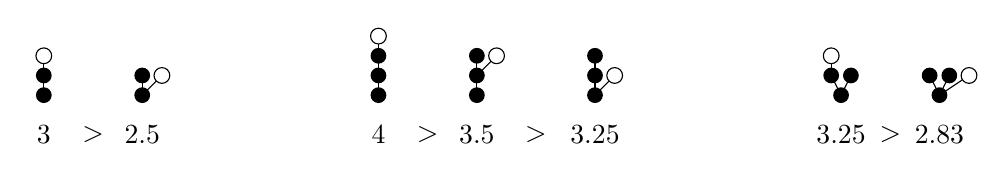
\begin{tikzpicture}[scale=0.25]
      \newcommand{\treeone}{
        \fill(0,0) circle (0.4);
        \fill(0,1) circle (0.4);
        \fill(0,2) circle (0.4);
        \draw(0,0) -- (0,1);
        \draw(0,1) -- (0,2);
      }
      \newcommand{\treetwo}{
        \fill(0,0) circle (0.4);
        \fill(-.50,1) circle (0.4);
        \fill(.50,1) circle (0.4);
        \draw(0,0) -- (0.5,1);
        \draw(0,0) -- (-.5,1);
      }
      \newcommand{\treethree}{
        \fill(0,0) circle (0.4);
        \fill(0,1) circle (0.4);
        \draw(0,0) -- (0,1);
      }
      % \begin{scope}
      %   \treeone;
      % \end{scope}
      % \begin{scope}[xshift=9cm]
      %   \treetwo;
      % \end{scope}

      \begin{scope}[yshift=-5cm, xshift=-20.5cm]
        \begin{scope}
          \treethree;
          \draw(0,1) -- (0,2);
          \draw[fill=white](0,2) circle (0.4);
          \node at (0,-2) {3};
        \end{scope}
        \node at (2.5,-2) {$>$};
        \begin{scope}[xshift=5cm]
          \treethree;
          \draw(0,0) -- (1,1);
          \draw[fill=white](1,1) circle (0.4);
          \node at (0,-2) {2.5};
        \end{scope}
      \end{scope}

      \begin{scope}[yshift=-5cm, xshift=-3.5cm]
        \begin{scope}
          \treeone;
          \draw(0,2) -- (0,3);
          \draw[fill=white](0,3) circle (0.4);
          \node at (0,-2) {4};
        \end{scope}
        \node at (2.5,-2) {$>$};
        \begin{scope}[xshift=5cm]
          \treeone;
          \draw(0,1) -- (1,2);
          \draw[fill=white](1,2) circle (0.4);
          \node at (0,-2) {3.5};
        \end{scope}
        \node at (8,-2) {$>$};
        \begin{scope}[xshift=11cm]
          \treeone;
          \draw(0,0) -- (1,1);
          \draw[fill=white](1,1) circle (0.4);
          \node at (0,-2) {3.25};
        \end{scope}
        % \node at (4,-1.5) {$4 > 3.5 > 3.25$};
      \end{scope}

      \begin{scope}[yshift=-5cm, xshift=20cm]
        \begin{scope}[xshift=0cm]
          \treetwo;
          \draw(-.5,1) -- (-.5,2);
          \draw[fill=white](-.5,2) circle (0.4);
          \node at (0,-2) {3.25};
        \end{scope}
        \node at (2.5,-2) {$>$};
        \begin{scope}[xshift=5cm]
          \treetwo;
          \draw(0,0) -- (1.5,1);
          \draw[fill=white](1.5,1) circle (0.4);
          \node at (0,-2) {2.83};
        \end{scope}
      \end{scope}
      
    \end{tikzpicture}
    \caption{Adding new tasks to degenerate intrees with less than four nodes such that the resulting intrees are still degenerate. The original (2- resp. 3-node) intrees are drawn black, the newly added tasks are drawn white. Below each intree, we see the corresponding optimal expected run time. The lower the level of the newly added task, the lower the expected run time. This serves as basis for the induction proof for lemma \ref{lem:p3-adding-tasks-level-keep-scheduled-same-inequality}.}
    \label{fig:p3-lemma-adding-intrees-induction-start}
  \end{figure}

  If we add two tasks $z_1$ and $z_2$ with $level(z_1)>level(z_2)$ in a way such that the original ready tasks stay ready and the resulting intrees stay degenerate, we obtain the intrees depicted in figure \ref{fig:p3-lemma-adding-intrees-induction-start} (trees \emph{including} the white nodes). By simply computing the expected optimal run times, we can confirm our claim for intrees with 3 nodes.

  We now do the induction step by considering an intree with $n$ tasks. 
  Let $x,y$ be ready tasks and $z_1$ and $z_2$ to be added with $level(z_1) > level(z_2)$ such that the resulting intrees are degenerate.
  We can now compare the two runs that can occur if $x,y,z_1$ resp. $x,y,z_2$ are initially scheduled. 
  Therefore, we consider what happens in $I_1=I\cup\left\{ z_1 \right\}$ resp. $I_2=I\cup\left\{ z_2 \right\}$ if either $x$, $y$ or $z_1/z_2$ finishes first:

  \begin{itemize}
  \item If $z_1$ resp. $z_2$ is the first task to finish, the resulting intree is exactly $I$. Thus, the remaining run times for these cases are identical if the next task chosen is the same in both trees. We denote the task that may be chosen additionally to $x$ and $y$ by $z'$. If it is the case that only $x$ and $y$ can be scheduled, we set $z'=x$ to simplify notation. The corresponding run time for the resulting intree is then $T^*_{x,y,z'}(I)$.

  \item If $x$ is the first task to finish, then the resulting intrees are 
    \begin{equation*}
      I^x_{1}=I_1\setminus\left\{ x \right\} \quad \text{ resp. } \quad I^x_{2}=I_2\setminus\left\{ x \right\}.
    \end{equation*}

    By $x'$ we denote the task that is scheduled next in the optimal schedule for intree $I_1^x$. 
    If there are only two ready tasks left in $I_1^x$ (which then must be $y$ and $z_1$), we set $x'=y$. The expected optimal runtime for $I_1^x$ in this situaion is then given by $T_{x',y,z_1}^*(I_1^x)$.

    We now examine whether $x'$ is also ready in the intree $I_2^x$:
    \begin{itemize}
    \item If there are only two ready tasks left in $I_1$ (namely $x$ and $y$), we set -- as mentioned before -- $x'=y$. Thus, in $I_2^x$, $x'$ is still ready\footnote{It may even be the case that $I_2^x$ contains some additional ready tasks that are not ready in $I_1^x$.}.
    \item If $x'$ is the direct successor of $x$, then $x$ must have been the \emph{single topmost task} and the \emph{single predecessor} of $x'$ (since $I_1^x$ is a degenerate tree). However, since we assumed that $level(z_2)<level(z_1)$ and $z_1$ can not be a predecessor of $x'$ (since $x'$ is ready in $I_1$), it can not be the case that $z_2$ blocks $x'$ in $I_2^x$. We conclude that in this case $x'$ is ready in $I_2^x$.

      % Moreover, since $x'$ is ready in $I_1^x$, the task $z_1$ can not be a predecessor of $x'$. Since $level(z_2)<level(z_1)$ and since $I_1^x$ and $I_2^x$ are both degenerate intrees, $z_2$ can not block $x'$.\todo{Genauer ausführen. Evtl. auslagern.}
    \item If $x'$ is not the direct successor of $x$, we recognize the fact that $x'$ must reside on a certain level with in the degenerate intree. 

      If $x'$ is \emph{not} in the topmost level, it can not be blocked by $z_2$ because we assumed that $z_2$ is added in a way such that $I\cup\{z_2\}$ is still a degenerate intree.

      Otherwise (if $x'$ is a topmost task), $z_2$ can not be added \emph{above} $x'$ because we assumed $level(z_1)>level(z_2)$.

      Again, $x'$ is ready in $I_2^x$.
      % we still have two subcases:
      % \begin{itemize}
      % \item If there are other tasks at the same level as $x'$ (i.e. at the topmost level), then we can -- without loss of generality\footnote{Because of isomorphism.} -- assume that $z_2$ was added to another task on the same level as $x'$.
      % \item If $x'$ was the \emph{only} topmost task, then it \emph{might} be the case that $z_2$ was chosen in a way such that it is the direct predecessor of $x'$. In this case, we can argue that $level(z_1) > level(z_2)$ and, thus, know that $z_2$ can not block $x'$, because $x'$ is a topmost task.
      % \end{itemize}

      % $x'$ must be on a lower level then $x$ (because we are dealing with a degenerate intree). We assumed that we added $z_2$ in a manner such that $I_2=I\cup\left\{ z_2 \right\}$ is a degenerate subtree. Thus, $z_2$ could not have been added with $x'$ as its successor. Thus, $x'$ is not blocked by $z_2$ in $I_2$.
    \end{itemize}
    We observed that for $I_2^x$, the task $x'$ must be ready.
    
    The intrees $I^x_{1}$ and $I^x_{2}$ have exactly $n$ tasks -- and they have a common subtree, namely
    \begin{equation*}
      I^x := I^x_{1}\setminus\left\{ z_1 \right\}=I^x_{2}\setminus\left\{ z_2 \right\}.
    \end{equation*}

    
    We can now apply the induction hypothesis for the intree $I^x$, since this intree contains only $n-1$ tasks: We have an intree with $n-1$ tasks (namely $I^x$) and two tasks $z_1$ and $z_2$ with $level(z_1)>level(z_2)$, $I^x_1 = I^x\cup\left\{ z_1 \right\}$ and $I^x_2 = I^x\cup\left\{ z_2 \right\}$, implying that $T^*_{x',y,z_1}(I^x_1)>T^*_{x',y,z_2}(I^x_{2})$.
  \item If $y$ is the first task to finish, we argue similar to the $x$ case, thereby considering $I^y_{1},I^y_{2}$ and $I^y$ which are all defined analogously. This finally yields the following inequality: $T^*_{x,y',z_1}(I^y_{1}) > T^*_{x,y',z_2}(I^y_{2})$.
  \end{itemize}

  The above considerations are illustrated in figure 
\ref{fig:p3-adding-tasks-level-keep-scheduled-same-inequality}.\todo{Figure anpassen!}
  
  \begin{figure}[t]
    \centering
    \newcommand{\drawx}{
      \node[draw=black,circle] at (.9,3) {$x$};
    }
    \newcommand{\drawxx}{
      \node[draw=black,circle] at (.7,2) {$x'$};
    }
    \newcommand{\drawy}{
      \node[draw=black,circle] at (-1.5,4) {$y$};
    }
    \newcommand{\drawyy}{
      \node[draw=black,circle] at (-1.5,3) {$y'$};
    }
    \newcommand{\rawtriangle}{
      \draw
      [dotted, very thick,
      %fill=white!90!black, 
      rounded corners]
      (0,0) -- (3,2) -- (3.5,8) -- (-3.5,8) -- (-3,2) -- cycle;
    }
    \newcommand{\treetriangle}{
      \rawtriangle;
      \drawx;
      \drawy;
    }
    \newcommand{\abstand}{7.5cm}
    \begin{tikzpicture}[scale=.4]
      \begin{scope}[xshift=-\abstand]
        \treetriangle
        \node[draw=black,circle] at (0,6.5) {$z_1$};
      \end{scope}
      \begin{scope}[xshift=\abstand]
        \treetriangle
        \node[draw=black,circle] at (1,5) {$z_2$};
      \end{scope}
      
      \begin{scope}[xshift=-2*\abstand, yshift=-9cm]
        \rawtriangle
        \node[draw=black,circle] at (0,6.5) {$z_1$};
        \drawxx;
        \drawy;
      \end{scope}

      \begin{scope}[xshift=-\abstand, yshift=-9cm]
        \rawtriangle
        \node[draw=black,circle] at (0,6.5) {$z_1$};
        \drawx;
        \drawyy;
      \end{scope}

      \begin{scope}[xshift=0, yshift=-9cm]
        \treetriangle
        \node[draw=black,circle] at (.3,5.5) {$z'$};
      \end{scope}
      
      \begin{scope}[xshift=\abstand, yshift=-9cm]
        \rawtriangle
        \node[draw=black,circle] at (1,5) {$z_2$};
        \drawxx;
        \drawy;
      \end{scope}

      \begin{scope}[xshift=2*\abstand, yshift=-9cm]
        \rawtriangle
        \node[draw=black,circle] at (1,5) {$z_2$};
        \drawx;
        \drawyy;
      \end{scope}
      
      \draw[thick,->](-\abstand,0) -- +(0,-.8);
      \draw[thick,->](-\abstand-2cm,1) -- +(-\abstand+4cm,-1.6);
      \draw[thick,->](-\abstand+2cm,1) -- +(\abstand-4cm,-1.6);

      \begin{scope}[xshift=2*\abstand]
        \draw[thick,->](-\abstand,0) -- +(0,-.8);
        \draw[thick,->](-\abstand-2cm,1) -- +(-\abstand+4cm,-1.6);
        \draw[thick,->](-\abstand+2cm,1) -- +(\abstand-4cm,-1.6);
      \end{scope}
      
      % legend      
      \draw[decoration=brace,decorate=true](-11,8.25) --node[above]{$I_1$} +(7,0);
      \draw[decoration=brace,decorate=true](  4,8.25) --node[above]{$I_2$} +(7,0);
      \draw[decoration={brace,mirror},decorate=true](  -18,-9.5) --node[below, yshift=-.2cm]{$I^x_{1}$} +(6,0);
      \draw[decoration={brace,mirror},decorate=true](-10.5,-9.5) --node[below, yshift=-.2cm]{$I^y_{1}$} +(6,0);
      \draw[decoration={brace,mirror},decorate=true](   -3,-9.5) --node[below, yshift=-.2cm]{$I$} +(6,0);
      \draw[decoration={brace,mirror},decorate=true](  4.5,-9.5) --node[below, yshift=-.2cm]{$I^x_{2}$} +(6,0);
      \draw[decoration={brace,mirror},decorate=true](   12,-9.5) --node[below, yshift=-.2cm]{$I^y_{2}$} +(6,0);
    \end{tikzpicture}

    \caption{Proof sketch for lemma \ref{lem:p3-adding-tasks-level-keep-scheduled-same-inequality}. By induction hypothesis, we have that $T^*_{x',y,z_1}(I^x_{1}) > T^*_{x',y,z_2}(I^x_{2})$ and $T^*_{x,y',z_1}(I^y_{1}) > T^*_{x,y',z_2}(I^y_{2})$, from which we deduce $T^*_{x,y,z_1}(I_1) > T^*_{x,y,z_2}(I_2)$. Note that $z_2$ can not block $x'$ or $y'$ since $z_1$ didn't block any of the two and we required that adding $z_1$ resp. $z_2$ still results a degenerate tree.}
    \label{fig:p3-adding-tasks-level-keep-scheduled-same-inequality}
  \end{figure}
  
  Now we argue that the run times for $I_1$ and $I_2$ can be computed as follows:
  \begin{align*}
    T^*_{x,y,z_1}(I_1) & = 
      \frac{1}{3} + 
      \frac{1}{3}\cdot \left( 
        T_{x,y,z'}^*(I) + 
        T^*_{x',y,z_1}(I^x_{1}) +
        T^*_{x,y',z_1}(I^y_{1}) 
      \right)
      \\
    T^*_{x,y,z_2}(I_2) & = 
      \frac{1}{3} + 
      \frac{1}{3}\cdot \left( 
        T_{x,y,z'}^*(I) + 
        T^*_{x',y,z_2}(I^x_{2}) +
        T^*_{x,y',z_2}(I^y_{2}) 
      \right)
  \end{align*}

  We will now use the aforementioned inequalities $T^*_{x',y,z_1}(I^x_{1}) > T^*_{x',y,z_2}(I^x_{2})$ and $T^*_{x,y',z_1}(I^y_{1}) > T^*_{x,y',z_2}(I^y_{2})$:
\begin{align*}
    T^*_{x,y,z_1}(I_1) & = 
      \frac{1}{3} + 
      \frac{1}{3}\cdot \left( 
        T_{x,y,z'}^*(I) + 
        T^*_{x',y,z_1}(I^x_{1}) +
        T^*_{x,y',z_1}(I^y_{1}) 
      \right)
      > 
      \\
      & >
      \frac{1}{3} + 
      \frac{1}{3}\cdot \left( 
        T_{x,y,z'}^*(I) + 
        T^*_{x',y,z_2}(I^x_{2}) +
        T^*_{x,y',z_2}(I^y_{2}) 
      \right) 
      = T^*_{x,y,z_2}(I_2).
  \end{align*}

  This proves our claim for $level(z_1) > level(z_2)$. It is simple to obtain the claim for the version where $level(z_1) \geq level(z_2)$: If the levels are the same, the resulting degenerate intrees $I_1$ and $I_2$ are isomorphic (and there is an isomorphism that maps $z_1$ onto $z_2$), thus the optimal run time is the same. If the levels are different, we argument as in the beginning of the proof.
\end{proof}

\paragraph{Application of lemma \ref{lem:p3-adding-tasks-level-keep-scheduled-same-inequality}}

We presented lemma \ref{lem:p3-adding-tasks-level-keep-scheduled-same-inequality} in a way that involved adding tasks to a certain intree, because this related well to our proof technique. In practice, we can use it to compare two degenerate intrees with $n$ nodes and that have a common subtree containing $n-1$ nodes.

We can now derive the following theorem.

\begin{theorem}
  Degenerate intrees are optimally scheduled by HLF.
\end{theorem}

\begin{proof}
  Consider a degenerate intree with $n=3$ tasks. It is trivially clear that for P3, a HLF schedule is optimal for this intree (see figure \ref{fig:p3-lemma-adding-intrees-induction-start} to see what these intrees look like -- we simply can conclude examine all possible schedules and see that the optimal ones is exactly HLF).
  
  Consider now a degenerate tree $I$ with $n$ nodes and assume that we know that for all degenerate trees with $n-1$ nodes HLF is optimal for three processors. If $I$ has two or less topmost tasks, it is obvious that we have to use HLF (since we can use at most two processors and HLF is known to be optimal for two processors --- see chapter \ref{chap:p2}).

  Thus, we only have to focus on the case where $I$ has at least three ready tasks.

  If we choose three topmost tasks $x,y,z$ of $I$, we can argue as follows: If $x$ is the task that finishes first, for the resulting subtree $I\setminus \left\{ x \right\}$, we can be sure that we can choose the next task such that we adhere to HLF, thus choosing the optimal solution for $I\setminus\left\{ x \right\}$ (by induction hypothesis). The same holds if $y$ or $z$ finishes first.
  
  We now consider a (possibly) non-HLF schedule for $I$ and compare it to the HLF schedule described before.
  Let $x',y',z'$ be the tasks to be chosen such that at least $x\neq x'$ or $y\neq y'$ or $z\neq z'$. We can -- without loss of generality -- assume $level(x')\leq level(x)$, $level(y')\leq level(y')$, $level(z')\leq level(z)$. If $x'$ is the first task to finish, we consider the degenerate intree $I\setminus\left\{ x' \right\}$. Since $I \setminus \left\{ x' \right\}$ is a degenerate intree with $n-1$ tasks, it would be optimal to use HLF. However, using HLF may or may not be possible depending on our previous choices of $y'$ and $z'$. That is, the optimum for $I\setminus\left\{ x' \right\}$ \emph{might} be acchieved if we chose $y'$ and $z'$ accordingly. From this we can conclude that the optimal expected run time is at least $T_{HLF}\left( I\setminus\left\{ x' \right\} \right)$, where $T_{HLF}$ denotes the run time for HLF (which we know, by induction, is optimal).

  Now we compare the run time for $I\setminus\left\{ x' \right\}$ to the optimal run time for $I \setminus\left\{ x \right\}$, which is exactly given by $T_{HLF}\left( I \setminus\left\{ x \right\} \right)$. We recognize that $I\setminus\left\{ x' \right\}$ and $I\setminus\left\{ x \right\}$ have a common subtree, namely $I\setminus\left\{ x,x' \right\}$ with $n-2$ tasks.
  
  Moreover, we know that for both $I\setminus\left\{ x \right\}$ and $I\setminus\left\{ x' \right\}$ HLF is optimal (because of our induction hypothesis) and that for $I\setminus\left\{ x \right\}$ and $I\setminus\left\{ x' \right\}$ both $y$ and $z$ must be in the optimal (i.e. HLF) schedule since $y$ and $z$ are two of the three topmost tasks. At last, we have $level(x) \geq level(x')$.
  Thus, we can apply lemma \ref{lem:p3-adding-tasks-level-keep-scheduled-same-inequality} for the degenerate tree $I\setminus \{x,x'\}$ with tasks $y$ and $z$ and deduce that
  \begin{equation*}
    T_{x',y,z}(I\setminus\{x\}) 
    \leq 
    \underbrace{T_{x,y,z}(I\setminus\{x'\})}_{\text{Optimal for $I\setminus \{x'\}$}}.
  \end{equation*}
  Equality holds if $x$ and $x'$ are on the same level.

  As stated before, for the intree $I\setminus\{x'\}$, the schedule chosen \emph{might} be a non-HLF schedule. In this case, the schedule performs even worse than $T_{x,y,z}(I\setminus\{ x'  \})$, since the optimal schedule would choose $x,y,z$ as scheduled tasks. This means that
  \begin{equation*}
    T_{x,y,z}(I\setminus\{x'\})
    \leq
    T_{x'',y',z'}(I\setminus\{x'\}),
  \end{equation*}
  where $x''$ is the task chosen by the non-HLF schedule, finally implying (by $T_{HLF}(I\setminus\{x\}) \leq T_{x',y,z}\left( I\setminus\left\{ x \right\} \right)$) that
  \begin{equation*}
    T_{HLF}(I\setminus\{x\})
    \leq
    T_{x'',y',z'}(I\setminus\{x'\}).
  \end{equation*}
  %because the HLF schedule is at least as good as the schedule that starts out with tasks $x',y,z$.
  We argue similar for tasks $y$ and $y'$ resp. $z$ and $z'$ and finally obtain the following:

  \begin{eqnarray*}
    T_{x',y,z}(I\setminus\{x\})
    & \leq &
    T_{x'',y',z'}(I\setminus\{x'\}) \\
    T_{x,y',z}(I\setminus\{y\})
    & \leq &
    T_{x',y'',z'}(I\setminus\{y'\}) \\
    T_{x,y,z'}(I\setminus\{z\})
    & \leq &
    T_{x',y',z''}(I\setminus\{z'\}) \\
  \end{eqnarray*}
  Note that if e.g. $x=x'$, the above three equations are still satisfied.
  Combining the above inequalities yields that
  \begin{eqnarray*}
    %T_{HLF}(I) = 
    T_{x,y,z}(I) 
    & \leq & 
    \frac{1}{3} + \frac{1}{3} \cdot 
    \left( 
      T_{x',y,z}(I\setminus\{x\}) +
      T_{x,y',z}(I\setminus\{y\}) +
      T_{x,y,z'}(I\setminus\{z\})
    \right) 
    \leq \\
    & \leq &
    \frac{1}{3} + \frac{1}{3} \cdot 
    \left( 
      T_{x'',y',z'}(I\setminus\{x'\}) +
      T_{x',y'',z'}(I\setminus\{y'\}) +
      T_{x',y',z''}(I\setminus\{z'\})
    \right) \leq \\
    & \leq &
    T_{x',y',z'}(I)
  \end{eqnarray*}

  This finally shows that a HLF schedule is at least as good as an arbitrary other task, meaning that HLF is optimal for three processors on degenerate trees.
\end{proof}

\section{Parallel chains}
\label{sec:p3-parallel-chains}

We will now consider another class of intrees that can be shown to have HLF as optimal schedules.

\begin{definition}[Parallel chain]
  Let $I$ be an intree. We call $I$ a \emph{parallel chain}, if each task except the root has at most one predecessor. The root may have arbitrarily many predecessors.
\end{definition}

We show an example of a parallel chain in figure \ref{fig:parallel-chain-intro-figure}.

\begin{figure}[th]
  \centering
  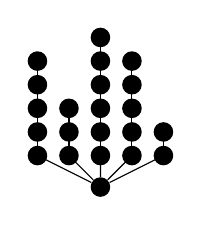
\begin{tikzpicture}[scale=.2]
    \foreach \y in {1,...,5}
    \node[circle, scale=0.75, fill]() at (0,\y*1.5){};
    \foreach \y in {1,...,3}
    \node[circle, scale=0.75, fill]() at (2,\y*1.5){};
    \foreach \y in {1,...,6}
    \node[circle, scale=0.75, fill]() at (4,\y*1.5){};
    \foreach \y in {1,...,5}
    \node[circle, scale=0.75, fill]() at (6,\y*1.5){};
    \foreach \y in {1,...,2}
    \node[circle, scale=0.75, fill]() at (8,\y*1.5){};
    \node[circle, scale=0.75, fill] (tid0) at (4,-.5){};
    \draw (0,1.5) -- (0, 7.5);
    \draw (2,1.5) -- (2, 4.5);
    \draw (4,1.5) -- (4, 9);
    \draw (6,1.5) -- (6, 7.5);
    \draw (8,1.5) -- (8, 3.5);
    \foreach \x in {0,...,4}
    \draw (tid0) -- (\x*2, 1.5);
  \end{tikzpicture}
  \caption{Parallel chains have the property that -- except for the root -- all tasks have at most one direct predecessor. Note that for parallel chains, HLF admits no ambiguities in the sense that all different possible choices of HLF result in equivalent snapshots.}
  \label{fig:parallel-chain-intro-figure}
\end{figure}

\subsection{Parallel chains are optimally scheduled by HLF}
\label{sec:parallel-chains-optimally-hlf}

We start out by a lemma that we will use later. This lemma is an analogue variant of a lemma described in \cite{chandyreynoldsshortpaper1975}. While their lemma works for two processors and general intrees, our variant is for three processors, but restricted to parallel chains.

\begin{lemma}
  \label{lemma:parallel-chains-flatness}
  Let $I$ be an intree and $x$ and $y$ two ready tasks with $level(x) > level(y)$. Then, $T_{HLF}(I\setminus\{ x \}) < T_{HLF}(I\setminus\{ y \})$, where $T_{HLF}(I)$ denotes the run time that is acchieved if intree $I$ is scheduled according to HLF.
\end{lemma}

\begin{proof}
  \newcommand{\iminus}[1]{I\setminus\{#1\}}

  We prove the claim by induction. For parallel chains with fewer than 6 tasks (all parallel chains with fewer than 5 tasks are trivially optimally scheduled by HLF), the fact can be easily proven. Note that it suffices to examine all parallel chains with at least 3 ready tasks, since intrees with two or less tasks are optimally scheduled by HLF (according to the fact that only two processors can be used for those intrees and the fact that for two processors HLF is optimal). The only parallel chain with fewer than 6 tasks is the intree $(0,0,0,1)$. This parallel chain (and its resulting parallel chains after removing topmost tasks) are shown in figure       \ref{fig:parallel-intrees-lemma-induction-start-concrete}.

  \begin{figure}[th]
    \centering
    \begin{subfigure}{.38\textwidth}
      \centering
      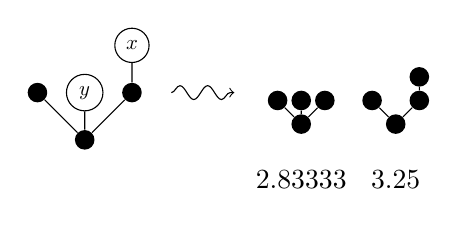
\begin{tikzpicture}[scale=.4]
        \node[circle, scale=0.75, fill] (tid0) at (2.25,1.5){};
        \node[circle, scale=0.75, fill] (tid1) at (0.75,3){};
        \node[circle, scale=0.75, draw] (tid2) at (2.25,3){$y$};
        \node[circle, scale=0.75, fill] (tid3) at (3.75,3){};
        \node[circle, scale=0.75, draw] (tid4) at (3.75,4.5){$x$};
        \draw[](tid3) -- (tid4);
        \draw[](tid0) -- (tid1);
        \draw[](tid0) -- (tid2);
        \draw[](tid0) -- (tid3);
        \draw[->, decorate, decoration=snake](5,3) -- (7,3);
        \begin{scope}[xshift=8cm, scale=.5, yshift=2.5cm]
          \node[circle, scale=0.75, fill] (tid0) at (2.25,1.5){};
          \node[circle, scale=0.75, fill] (tid1) at (0.75,3){};
          \node[circle, scale=0.75, fill] (tid2) at (2.25,3){};
          \node[circle, scale=0.75, fill] (tid3) at (3.75,3){};
          \draw[](tid0) -- (tid1);
          \draw[](tid0) -- (tid2);
          \draw[](tid0) -- (tid3);
          \node at (2.25,-2){2.83333};
        \end{scope}
        \begin{scope}[xshift=11cm, scale=.5, yshift=2.5cm]
          \node[circle, scale=0.75, fill] (tid0) at (2.25,1.5){};
          \node[circle, scale=0.75, fill] (tid1) at (0.75,3){};
          \node[circle, scale=0.75, fill] (tid3) at (3.75,3){};
          \node[circle, scale=0.75, fill] (tid4) at (3.75,4.5){};
          \draw[](tid3) -- (tid4);  
          \draw[](tid0) -- (tid1);
          \draw[](tid0) -- (tid3);
          \node at (2.25,-2){3.25};
        \end{scope}
      \end{tikzpicture}
      \caption{Original parallel chain $(0,0,0,1)$, and the parallel chains resulting from removing $x$ resp. $y$ with their respective expected HLF run times. This serves as base case for the induction in the proof of lemma \ref{lemma:parallel-chains-flatness}.}
      \label{fig:parallel-intrees-lemma-induction-start-concrete}
    \end{subfigure}
    \quad
    \caption{Removing tasks on lower levels from parallel chains results in higher run times than removing tasks on higher levels.}
    \label{fig:parallel-intrees-lemma-induction-start}
  \end{figure}

  We consider the HLF schedules on the intrees $I\setminus \{x\}$ and $I \setminus \{y\}$, with variable names as aforementioned. Note that the intrees $I\setminus \{x\}$ and $\setminus \{y\}$ have at least two common HLF-tasks (i.e. tasks that are scheduled by HLF). We call these two tasks $x_1$ and $x_2$. For the intree $\iminus{x}$, we call the third HLF-task $x_3$ and can compute its expected run time (for HLF) by
  \begin{equation*}
    T_{HLF}(\iminus{x}) = 
    \frac{1}{3} \cdot T(\iminus{x, x_1}) +
    \frac{1}{3} \cdot T(\iminus{x, x_2}) +
    \frac{1}{3} \cdot T(\iminus{x, x_3})
    .
  \end{equation*}
  On the other hand, for the intree $\iminus{y}$, we call the third HLF-task $x'$ and can compute its expected run time analogously by
  \begin{equation*}
    T_{HLF}(\iminus{y}) = 
    \frac{1}{3} \cdot T(\iminus{y, x_1}) +
    \frac{1}{3} \cdot T(\iminus{y, x_2}) +
    \frac{1}{3} \cdot T(\iminus{y, x'})
    .
  \end{equation*}
  We can now compare $T(\iminus{x, x_1})$ with $T(\iminus{y, x_1})$, $T(\iminus{x, x_2})$ with $T(\iminus{x, x_2})$ and $T(\iminus{x, x_3})$ with $T(\iminus{y, x'})$.
  
  The intrees $\iminus{x,x_1}$ and $\iminus{y,x_1}$ have a common subtree, namely $\iminus{x_1}$. By induction ($\iminus{x_1}$ has $n-1$ tasks, $level(x) > level(y)$), we know that the expected HLF run time for $\iminus{x,x_1}$ is less than the expected run time for $\iminus{y,x_1}$. Note that $\iminus{x, x_1}$ has at least as many ready tasks as $\iminus{y,x_1}$. So, if $\iminus{y,x_1}$ has two or less ready tasks, the claim is true, because it has been shown for two processors in \cite{chandyreynoldsshortpaper1975} and we -- moreover -- can use a third processor for$\iminus{x,x_1}$. This consideration can be done for $x_2$ in the same manner. 

  It remains to compare $T(\iminus{x, x_3})$ and $T(\iminus{y, x'})$. If $\iminus{y,x'}$ has fewer ready tasks than $T(\iminus{x, x_3})$, then we trivially have $T(\iminus{x, x_3}) \leq T(\iminus{y, x'})$ (similar to the case before, it has been shown for two processors, and we additionally can use a third processor for $\iminus{x,x_3}$). We, thus, focus on other cases.

  \begin{itemize}
  \item  If $level(x')=level(x_3)$, the intrees $\iminus{x'}$ and $\iminus{x_3}$ are isomorphic (we are dealing with parallel chains only), and can -- thus -- be considered equal in our computations (we can do so because HLF can be seen as deterministic for parallel chains). That is, we can w.l.o.g. assume $x'=x_3$ if the levels of $x'$ and $x_3$ are equal. In this case, we have that $T(\iminus{x, x_3})$ and $T(\iminus{y, x'})$ share a common supertree (namely $\iminus{x_3}=\iminus{x'}$), and we know -- by induction since $level(x)>level(y)$ that $T(\iminus{x, x_3}) < T(\iminus{y, x'})$.
  \item   If $level(x') \neq level(x_3)$, we know that $x_3$ is \emph{not} a HLF task in $\iminus{y}$, but $x'$ is. This means that $x'$ can only be a HLF task since it is not part of $\iminus{y}$. Therefore, we conclude that $y$ must be the same as $x_3$ (implying w.l.o.g. $\iminus{x,y}=\iminus{y,x'}$). This means that $level(x)>level(y)=level(x_3)$. Moreover, because $x'$ is only a HLF task because $x_3$ is not existent in $\iminus{y}$, we know that $level(x') < level(x_3)$. Combining the inequalities yields $level(x)>level(x')$. We can now argue that $\iminus{y}$ is (w.l.o.g.) a common supertree of $\iminus{x,y}=\iminus{x,x_3}$ and $\iminus{y,x'}$ with $n-1$ tasks. Since -- as explained before -- $level(x) > level(x_3)$, we can apply the induction hypothesis and conclude that $T(\iminus{x, x_3}) \leq T(\iminus{y, x'})$.
  \end{itemize}

  We have now shown, that in any case the following hold:
  \begin{eqnarray*} 
    T(\iminus{x, x_1}) \leq T(\iminus{y, x_1}) \\
    T(\iminus{x, x_2}) \leq T(\iminus{x, x_2}) \\
    T(\iminus{x, x_3}) \leq T(\iminus{y, x'})
  \end{eqnarray*}
  These inequalities can be used to derive the desired inequality.
\end{proof}

\emph{Remark:} In the above proof, we used the fact that, for parallel chains, HLF does not admit any ambiguities (i.e. all tasks that can be chosen by HLF as the next task to be scheduled result in equivalent snapshots). We used this fact in the case distinction where we said that two intrees are isomorphic and we can consider them equal for our computations. This, however, is something that can not be extended to arbitrary intrees for three processors.

We will now use lemma \ref{lemma:parallel-chains-flatness} to derive the following theorem.

\begin{theorem}
  Parallel chains are optimally scheduled by HLF.
\end{theorem}

\begin{proof}
  \newcommand{\iminus}[1]{I\setminus\{#1\}}

  We prove the claim by induction and can clearly observe that for any parallel chain with fewer than 5 tasks, HLF is optimal (because there is no other possibility to schedule the tasks).
  
  Consider the HLF run time for a parallel chain $I$ with $n$ tasks. Let $x_1,x_2,x_3$ denote the HLF tasks of $I$. We can compute the expected run time by
  \begin{equation*}
    T_{HLF}(I) = 
    \frac{1}{3} \cdot T(\iminus{x_1}) +
    \frac{1}{3} \cdot T(\iminus{x_2}) +
    \frac{1}{3} \cdot T(\iminus{x_3})
    .
  \end{equation*}
  For the parallel chains $\iminus{x_1}, \iminus{x_2}$ and $\iminus{x_3}$ (each having $n-1$ tasks) we know by induction that they are optimally scheduled by HLF. Note that -- if we start in an HLF manner -- we can choose the next tasks in a way such that for each of these intrees we behave according to HLF (because $x_1, x_2$ and $x_3$ are HLF tasks of $I$). This means, we can acchieve optimal run times for each of the three intrees.

  Now consider any other initial choice of tasks $y_1,y_2,y_3$. We can (w.l.o.g.) assume that $level(y_i)\leq level(x_i)$ for $i=1,2,3$ and we can assume (w.l.o.g.) $level(y_1) < level(x_1)$. The optimal expected run time for this initial choice of tasks is given by
  \begin{equation*}
    T_{\{y_1,y_2,y_3\}}(I) = 
    \frac{1}{3} \cdot T_{\{y_2,y_3,z_1\}}(\iminus{y_1}) +
    \frac{1}{3} \cdot T_{\{y_1,y_3,z_2\}}(\iminus{y_2}) +
    \frac{1}{3} \cdot T_{\{y_1,y_2,z_3\}}(\iminus{y_3})
    ,
  \end{equation*}
  where $z_i$ denotes the optimal task to be chosen if $y_i$ is the first task to finish and the expected run times noted above are the optimal ones that can be acchieved. We set $z_i$ to $y_{i+1(\mod 3)}$ if there are only two ready tasks in a subtree.
  
  We now apply lemma \ref{lemma:parallel-chains-flatness}: The parallel chains $\iminus{y_1}$ and $\iminus{x_1}$ share $I$ as common supertree and $level(x_1) > level(y_1)$. Applying the lemma shows that $T_{HLF}(\iminus{y_1}) > T_{HLF}(\iminus{x_1})$. We know by induction that $\iminus{y_1}$ is optimally scheduled by HLF, implying that $T_{y_2,y_3,z_1}(\iminus{y_1}) \geq T_{HLF}(\iminus{y_1})$. Combining the two inequalities gives $T_{y_2,y_3,z_1}(\iminus{y_1}) > t_{HLF}(\iminus{x_1})$.

  Similar to the proof of lemma \ref{lemma:parallel-chains-flatness}, we can argue that the parallel chain $\iminus{x_1}$ has at least as many ready task as $\iminus{y_1}$ and, thus, that $\iminus{x_1}$ has a lower expected HLF run time than $\iminus{y_1}$.

  The arguments work similar for $x_2$ resp. $x_3$ with $y_2$ resp. $y_3$ (where we can even allow the run times to be equal), resulting in our claim.

\end{proof}

\subsection{Comparison of exhaustive search and HLF}
\label{sec:parallel-chains-benchmarking}

Similarily to the comparison done in section \ref{sec:p3-degenerate-intrees}, we are interested in what we gain by the fact that parallel chains are optimally scheduled by HLF and, thus, need not be examined by an exhaustive search. 

To to this, we introduce a shorthand notation for parallel chains for this section: Instead of writing the whole intree in the usual manner, we focus on the lengths of the parallel chains. The parallel chain in figure \ref{fig:parallel-chain-intro-figure} consists of a root with five chains of lengths 5, 3, 6, 5 and 2. We simply write down the chain lengths as a tuple $(5,4,6,5,2)$.

The results are summed up in table \ref{tab:parallel-chains-comparison-leaf-hlf}. This table compares the scheduling approaches for parallel chains with a given amount of chains, where each chain has the same length. Other comparisons for selected parallel chains can be found in table \ref{tab:selected-parallel-chains-comparison}.

\begin{table}[ht]
  \centering
  \begin{subtable}{.45\textwidth}
    \centering
    \begin{tabular}[ht]{c|cccc}
      Length / No. chains & 3 & 4 & 5 & 6 \\
      \hline
      2 & 10 & 18 & 30 & 46 \\
      3 & 20 & 50 & 110 & 210 \\
      4 & 35 & 115 & 315 & 715 \\
      5 & 56 & 231 & 756 & 1981 \\
      6 & 84 & 420 & 1596 & 4732
    \end{tabular}
    \caption{Number of snapshots with examined by exhaustive search.}
  \end{subtable}
  \quad
  \begin{subtable}{.45\textwidth}
    \centering
    \begin{tabular}[ht]{c|cccc}
      Length / No. chains & 3 & 4 & 5 & 6 \\
      \hline
      2 & 10 & 14 & 18 & 22 \\
      3 & 20 & 30 & 40 & 50 \\
      4 & 35 & 55 & 75 & 95 \\
      5 & 56 & 91 & 126 & 161 \\
      6 & 84 & 140 & 196 & 252
    \end{tabular}
    \caption{Number of snapshots examined by HLF.}
  \end{subtable}
  \caption{Parallel chains: Comparison of the number of snapshots needed by exhaustive search in contrast to HLF. Each table denotes the number of chains to the right, and the length of each chain downwards.}
  \label{tab:parallel-chains-comparison-leaf-hlf}
\end{table}

\begin{table}[ht]
  \centering
  \begin{tabular}[ht]{lcc}
    Chain lengths & Exhaustive search & HLF \\
    \hline
    $(4,3,6,3)$ & 233 & 99 \\
    $(3,2,2,10)$ & 247 & 126 \\
    $(1,2,3,4)$ & 63 & 37 \\
    $(1,2,3,4,5)$ & 356 & 85 \\
    $(1,2,3,4,5,6)$ & 2007 & 172 \\
    $(1,2,3,4,5,6,7)$ & 10760 & 315
  \end{tabular}
  \caption{Comparing exhaustive search to HLF for selected parallel chains.}
  \label{tab:selected-parallel-chains-comparison}
\end{table}

We can see that (deterministic) HLF can drastically reduce the number of snapshots that have to be examined. This, of course, reduces computation times for parallel chains.

\section{Improving exhaustive search}
\label{sec:improving-exhaustive-search}

We have seen that degenerate intrees and parallel chains are optimally scheduled by HLF. We can now try to improve exhaustive search by proceeding according to (deterministic) HLF from the point on where we have a degenerate intree or a parallel chain. When we do so, we assume the following:

\emph{Assumption:} We assume that for degenerate intrees and parallel chains, that, if already two tasks are scheduled, the optimal task to be scheduled as third task should be chosen according to HLF.

Using this assumption, we can exclude snapshots that are non-HLF from the point on where the current intree is a degenerate trees or a parallel chain.

Please note that this assumption is not proven. Our experiments suggest that it is true. Also note that we possibly exclude too many snapshots, if the assumption turns out to be false. Nevertheless, we will use the assumption to research the number of snapshots that have to be examined by an improved exhaustive search. 

If we recognize that this improved exhaustive search performs significantly better than an ordinary exhaustive search, it might be worth proving (or possibly even disproving) the assumption. If not, it is probably not rewarding to examine whether the assumption is true or not (because our assumption (possibly) allows us to exclude more snapshots).



\section{Conclusion}
\label{sec:properties-schedules-conclusion}

We have seen two very regular classes of intrees that are optimally scheduled by HLF. Unfortunately, even simplest combinations of the two classes are not guaranteed to be optimally scheduled by HLF. As an example, consider the intree $(0,0,1,2,3,4,6,6,8,8)$ depicted in figure \ref{fig:hlf-vs-opt-0012346688} whose components attached to its root are a degenerate intree with 7 tasks and a simple chain with 3 tasks. As shown in section \ref{sec:p3-suboptimal-hlf-strictly-suboptimal}, for this intree, HLF is strictly suboptimal.

%%% Local Variables:
%%% TeX-master: "../thesis.tex"
%%% End: 